\documentclass[12pt]{article}
\usepackage{../../format}
\lhead{A Level Physics}
\usepackage{enumitem}
\setcounter{secnumdepth}{4}
\begin{document}
\begin{center}
\underline{\huge Paper 2 Cheat Sheet}
\end{center}
\section{Thermal physics}
\subsection{Thermal energy transfer}
\textbf{Specific heat capacity} - The energy required to raise the temperature of a unit mass of a given substance by one degree\\
\textbf{Specific latent heat}  - The energy required to change the state of a material without changing the temperature\\
\textbf{Temperature} - The average kinetic energy of the atoms or molecules in the system\\
\textbf{Heat} - Energy transfer due to a difference in temperature
\subsubsection{Continuous flow}
By dividing the specific heat capacity formula by t it can be found that
$$IV=mc\frac{\Delta T}{t}$$
This gives the power per second, where a mass $m$ flows in a time $t$
\subsection{Ideal gases}
{\renewcommand{\arraystretch}{2}
\begin{tabularx}{\textwidth}{|X|X|X|X|}
\hline
Law&Proportionality&Constant&Equation\\
\hline
Boyle's&$p\propto\dfrac{1}{v}$&Temperature, moles&$p_1v_1=p_2v_2$\\
\hline
Charles'&$V\propto T$&Pressure, moles&$\dfrac{v_1}{T_1}=\dfrac{v_2}{T_2}$\\
\hline
Gay-Lussac&$p\propto T$&Volume, moles&$\dfrac{p_1}{T_1}=\dfrac{p_2}{T_2}$\\
\hline
\end{tabularx}}
The two formulas on the formula book for the gas laws have $n$ moles and $N$ molecules
\subsubsection{Deriving Pressure volume work formula}
$$W=FS=F\times\Delta L=\frac{F}{A}\times A\Delta L=P\Delta V$$
\subsubsection{Types of masses}
\textbf{Molar mass} - The mass of a mole of a substance\\
\textbf{Molecular mass} - The mass of the molecules
\newpage
\subsection{Molecular kinetic theory model}
\subsubsection{Brownian motion as evidence for the existence of atoms}
\textbf{Brownian motion} - The random motion of smoke particles in a gas\\
As Newton's first law states that objects remain in motion until acted on by a force, the smoke particles should remain in motion, instead they move randomly, suggesting collisions with something else
\subsubsection{Explanation of relationships between p,V and T}
Increase pressure - More collisions, increase temperature. Same number of molecules, volume must decrease
\subsubsection{Empirical gas laws but theoretical kinetic theory}
By changing variables of a gas, the gas laws can be derived, however the kinetic theory is based on what else would be expected to be required to be constant.
\subsubsection{Derivation}
\textcolor{red}{Newton's $3^{\text{rd}}$ law - Every action has an equal and opposite reaction}\\
$\Delta mc=mc_{x1}--mc_{x1}=2mc_{x1}$\\
\\
\textcolor{red}{Use $\text{Velocity}=\dfrac{\text{Distance}}{\text{Time}}$}\\
Time=$\dfrac{\text{Distance}}{\text{Velocity}}=\dfrac{2l}{c_{x1}}$\\
\\
\textcolor{red}{Use force$=\dfrac{\text{Change in momentum}}{\text{time}}$}\\
$\text{Force}=\dfrac{\Delta mc}{\Delta t}=\dfrac{2mc{x1}}{2l/c_{x1}}=\dfrac{mc_{x1}^2}{l}$\\
\\
\textcolor{red}{Use Pressure$=\dfrac{\text{Force}}{\text{Area}}$}\\
\\
$p_1=\dfrac{mc_{x1}^2/l}{l^2}=\dfrac{mc_{x1}^2}{l^3}$\\
\\
\textcolor{red}{Expand for N particles}\\
$p=\Sigma p_n=p_1+p_2+p_3...+p_N$\\
\\
$p=\dfrac{mc_{x1}^2}{l^3}+\dfrac{mc_{x2}^2}{l^3}+\dfrac{mc_{x3}^2}{l^3}+\dfrac{mc_{xN}^2}{l^3}$\\
\\
$p=\dfrac{m}{l^3}(c_{x1}^2+c_{x2}^2+c_{x3}^2...+c_{xN}^2)$\\
\\
\textcolor{red}{The mean of all the squares of the velocities is written as $\mathlarger{\bar{c_x^2}}$}\\
\\
$\mathlarger{\bar{c_x^2}}=\dfrac{c_{x1}^2+c_{x2}^2+c_{x3}^2...+c_{xN}^2}{N}$\\
\\
$N\mathlarger{\bar{c_x^2}}=c_{x1}^2+c_{x2}^2+c_{x3}^2...+c_{xN}^2$\\
\\
\\
\textcolor{red}{Simplify expression for pressure}\\
$p=\dfrac{Nm\mathlarger{\bar{c_x^2}}}{l^3}$\\
\\
\textcolor{red}{Consider in 3 dimensions}\\
\\
$\mathlarger{\bar{c^2}=\bar{c_x^2}+\bar{c_y^2}+\bar{c_z^2}}$\\
\textcolor{red}{Average of mean square velocity for each dimension are equal}\\
\\
$\mathlarger{\bar{c_x^2}=\bar{c_y^2}=\bar{c_z^2}}$\\
\textcolor{red}{Simplify 3D formula}\\
\\
$\mathlarger{\dfrac{\bar{c^2}}{3}=\bar{c_x^2}=\bar{c_y^2}=\bar{c_z^2}}$\\
\\
\textcolor{red}{Simplify pressure formula}\\
\\
$p=\dfrac{1}{3}\times\dfrac{Nm\mathlarger{\bar{c^2}}}{l^3}$\\
\\
\textcolor{red}{Insert Density formula}\\
\\
$\rho=\dfrac{\text{Mass}}{\text{Volume}}=\dfrac{Nm}{l^3}$
\\
\textcolor{red}{Substitute into Pressure formula}\\
$$p=\frac{1}{3}\rho\mathlarger{\bar{c^2}}$$
\section{Fields and their consequences}
\subsection{Fields}
Similarities and differences between gravitational and electrostatic forces\\
\setitemize{noitemsep,topsep=-5pt,leftmargin=*}%Compress list
\begin{tabularx}{\textwidth}{|X|X|}
\hline
Similarities&Differences\\
\hline
\begin{itemize}
\item Inverse square laws
\item Use of field lines
\item Use of potential
\item Use of equipotentials
\end{itemize}& Masses always attract, but charges may attract or repel\\
\hline
\end{tabularx}
\newpage
\subsection{Gravitational fields}
\subsubsection{Gravitational field strength}
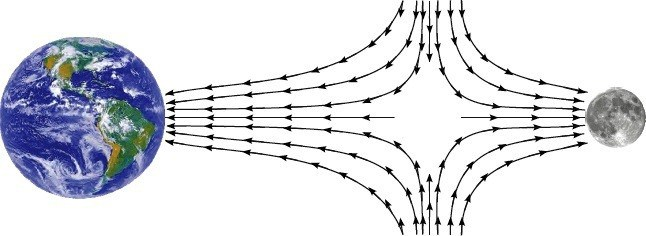
\includegraphics[width=8cm]{gravity.jpg}
\subsubsection{Gravitational potential}
Gravitational potential has a value of 0 at infinity, then reduces as it approaches the planet.\\
\textbf{Gravitational potential} - The work done in moving a unit mass from infinity to that point int he field\\
\textbf{Gravitational potential difference} - The work done in moving a unit mass from one point to another \\
\textbf{Equipotential} - The group of points with the same potential energy\\
\\
The sign is negative because a negative amount of work has to be done to move the object from infinity to earth because the object is attracted to earth.
\subsubsection{Orbits of planets and satellites}
\paragraph{Kepler's law}
$$F=\frac{GMm}{r^2}=\frac{mv^2}{r}\quad \therefore \frac{GM}{r}=v^2$$
$$v=\frac{s}{t}=\frac{2\pi r}{T}$$
$$v^2=\frac{4\pi^2r^2}{T^2}=\frac{GM}{r}$$
$$\frac{r^2}{T^2}=\frac{GM}{4\pi^2}$$
RHS is a constant
$$r^2\propto T^2$$
\paragraph{Escape velocity}
$$\frac{1}{2}mv^2=\frac{GMm}{r}\quad \therefore v=\sqrt{\frac{2GM}{r}}$$
$$g=\frac{GM}{r^2}\quad \therefore gr=\frac{GM}{r}$$
$$v=\sqrt{2gr}$$
\paragraph{Total energy of an orbiting satellite}
$$\textrm{Total energy=KE+GPE}$$
$$KE=\frac{1}{2}mv^2$$
$$\frac{GM}{r^2}=\frac{v^2}{r}\quad \therefore v^2=\frac{GM}{r}$$
$$KE=\frac{1}{2}m\frac{GM}{r}$$
$$GPE=mV \quad	V=-\frac{GM}{r} \quad \therefore E_p=-\frac{GMm}{r}$$
$$E_T=E_K+E_P=\frac{GMm}{2r}+-\frac{GMm}{r}=-\frac{GMm}{2r}$$
\paragraph{Synchronous orbits}
$ $\\
\textbf{Geosynchronous orbit} - Time period of 24h, will be seen at the same place at the same time every day\\ 
\textbf{Geostationary orbit} - Time period of 24h, but in the plane of the equator and travelling the same direction as the earth, appears stationary to an observer on the ground\\
\\
The height at which these satellites must be is determined by Kepler's law
\subsection{Electric fields}
\subsubsection{Coulomb's law}
This is the first equation under electric fields on the data sheet, it describes the force between two point charges in a vacuum\\
\textbf{Permittivity of free space} - The charge per unit area in coulombs per square metre on oppositely charged plates when the electric field strength between the plates is one volt per metre\\
The difference between the permittivity of free space and the permittivity of air is so insignificant air can be treated as a vacuum.\\
\textbf{Electric field strength} - At a point in an electric field, the force per unit charge on a small positively charged object in that field
\begin{center}
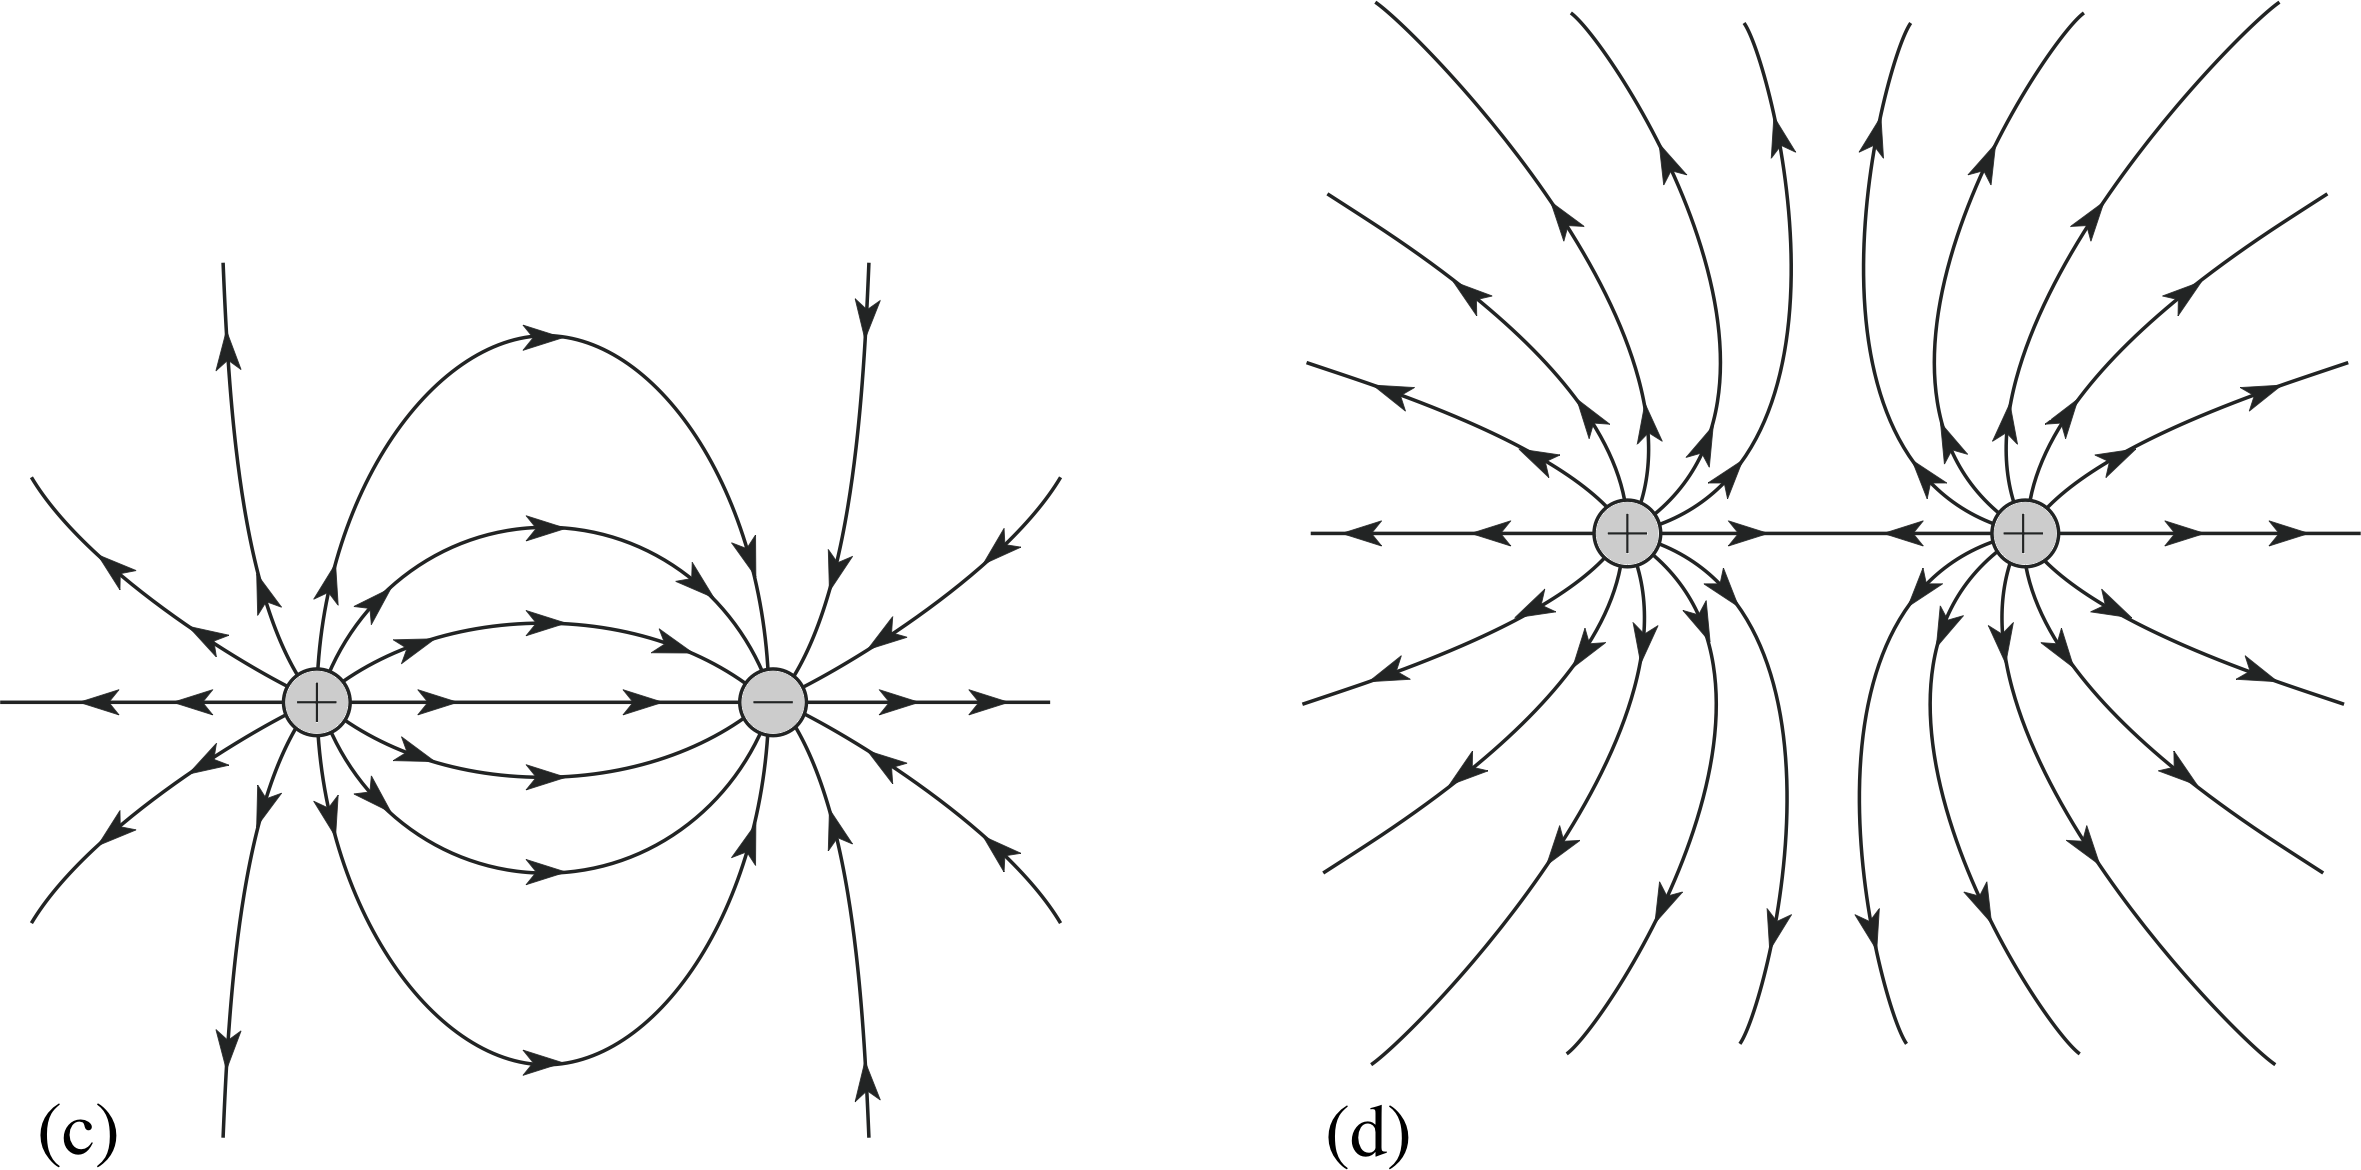
\includegraphics[width=12cm]{field_lines.png} 
\end{center}

\paragraph{Derive $Fd=Q\Delta V$}
$$F=EQ \quad E=\frac{V}{d} \quad\therefore F=\frac{QV}{d} \quad\therefore Fd=QV$$
\paragraph{Particle in a uniform electric field}
\begin{center}
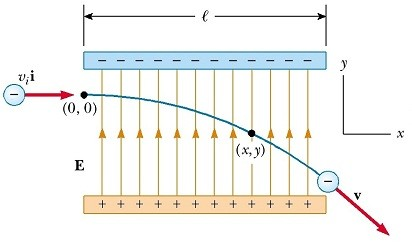
\includegraphics[width=8cm]{particle.jpg}
\end{center}
\end{document}